\documentclass[12pt]{article}
\usepackage[a4paper]{geometry}
\usepackage{fullpage}
\usepackage[T1]{fontenc}
\usepackage[utf8]{inputenc}
\usepackage{graphicx}
\usepackage{mathpazo}
\pagenumbering{gobble}
\usepackage{siunitx}
\DeclareSIUnit\voltampere{VA}
\usepackage{amsmath}
\usepackage[spanish]{babel}
\usepackage{steinmetz}
\usepackage{enumitem}
\usepackage{diffcoeff}

\renewcommand{\thesubsection}{Problema \arabic{subsection}}

\begin{document}

\title{}

\section{Transitorio de primer orden}

\subsection{}
En el circuito de la figura el interruptor ha estado abierto durante un tiempo
prolongado, y en el instante $t = 0$ se cierra. Hay que determinar las
respuestas del circuito en $t = 0^+$.

\begin{minipage}{0.5\linewidth}
  \center{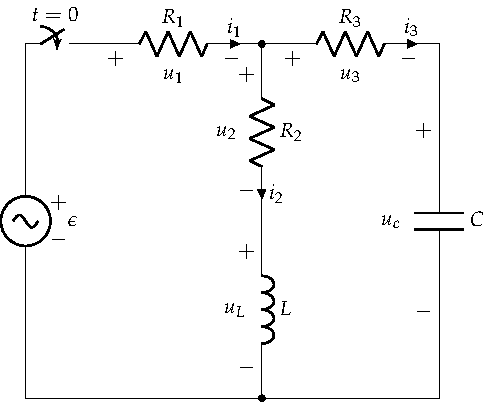
\includegraphics{figs/BT5_CondicionesIniciales_bobcon.pdf}}
\end{minipage}
\begin{minipage}{0.5\linewidth}
  \center{Datos:}
  \begin{align*}
    R1 &= 3\unit{\ohm}\\
    R2 &= 5\unit{\ohm}\\
    R3 &= 2\unit{\ohm}\\
    L &= 0,2\unit{\henry}\\
    C &= 0,5\unit{\milli\farad}\\
    \epsilon(t) &= 20\cos(t)\unit{\volt}
  \end{align*}
\end{minipage}

\subsubsection*{Solución}

En $t < 0$, dado que el interruptor ha estado abierto, la bobina y el condensador están descargados. Por tanto, $i_2(0^-) = \qty{0}{\ampere}$ y $u_C(0^-) = \qty{0}{\volt}$.

\smallskip
\begin{minipage}{0.6\linewidth}
En $t > 0$, al cerrarse el interruptor, la fuente de tensión alimenta al circuito. En el instante de cierre $e(0^+) = \qty{20}{\volt}$. Por otra parte, teniendo en cuenta las condiciones iniciales en la bobina y el condensador, tenemos:
\begin{align*}
  i_2(0^+) &= i_2(0^-) = \qty{0}{\ampere}\\
  u_C(0^+) &= u_C(0^-) = \qty{0}{\volt}
\end{align*}
Estos resultados implican que, en ese instante, la bobina se comporta como un circuito abierto y el condensador como un cortocircuito. 
\end{minipage}
\begin{minipage}{0.4\linewidth}
  \center{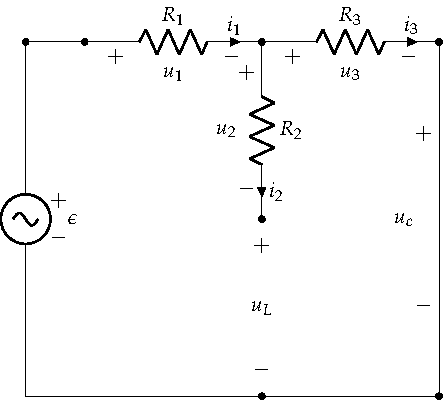
\includegraphics[scale=0.7]{figs/BT5_CondicionesIniciales_bobcon0+.pdf}}
\end{minipage}
\smallskip

En estas condiciones calculamos el resto de variables en $t = 0^+$.
\begin{align*}
  i_1(0^+) = i_3(0^+) &= \frac{e(0^+)}{R_1 + R_3} = \qty{4}{\ampere}\\
  u_1(0^+) &= R_1 \cdot i_1(0^+) = \qty{12}{\volt}\\
  u_2(0^+) &= R_2 \cdot i_2(0^+) = \qty{0}{\volt}\\
  u_3(0^+) &= R_3 \cdot i_3(0^+) = \qty{8}{\volt}\\
  u_L(0^+) &= u_3(0^+) = \qty{8}{\volt}
\end{align*}

\clearpage

\subsection{}

El interruptor de la figura ha estado cerrado por un tiempo muy
prolongado y en $t = 0$ se abre.

\begin{minipage}{0.5\linewidth}
  \center{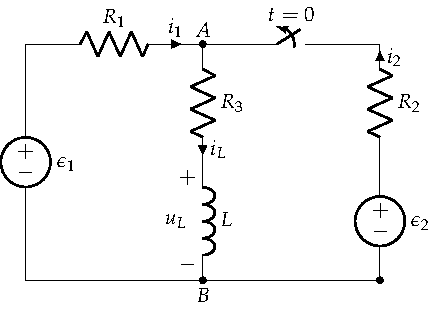
\includegraphics{figs/BT5_CondicionesIniciales_bobina.pdf}}
\end{minipage}
\begin{minipage}{0.5\linewidth}
  \center{Datos:}
  \begin{align*}
    R_1 &= \SI{5}{\ohm}\\
    R_2 &= \SI{5}{\ohm}\\
    R_3 &= \SI{2}{\ohm}\\
    L &= \SI{3.5}{\milli\henry}\\
    \epsilon_1 &= \SI{24}{\volt}\\
    \epsilon_2 &= \SI{12}{\volt}
  \end{align*}
\end{minipage}

\medskip

Con esta información se debe calcular:
\begin{enumerate}
\item Valores de $i_1(0^+)$, $i_2(0^+)$, $i_L(0+)$, $u_L(0^+)$ y
  $u_{AB}(0+)$.
\item Expresión de $i_L(t)$ para $t > 0$.
\item Expresiones de $u_L(t)$ y $u_{AB}(t)$ para $t > 0$.
\end{enumerate}

\subsubsection*{Solución}

En el circuito en $t <0$ la bobina se comporta como un
cortocircuito. Resolviendo por mallas el circuito resultante obtenemos
los valores para $t = 0^-$:

\begin{align*}
  i_L(0^-) &= \qty{4}{\ampere}\\
  i_1(0^-) &= \qty{3.2}{\ampere}\\
  i_2(0^-) &= \qty{0.8}{\ampere}
\end{align*}

En la bobina podemos plantear la condición de continuidad
$i_L(0^-) = i_L(0^+)$, que nos permite obtener los valores para
$t = 0^+$, una vez abierto el interruptor:

\begin{align*}
  i_L(0^+) &= \qty{4}{\ampere}\\
  i_1(0^+) &= i_L(0^+)\\
  i_2(0^+) &= \qty{0}{\ampere}\\
  u_L(0^+) &= \epsilon_1 - i_1(0^+) \cdot R_1 - i_L(0^+) \cdot R_3 = -\qty{4}{\volt}\\
  u_{AB}(0^+) &= \epsilon_1 - i_1(0^+) \cdot R_1 = \qty{4}{\volt}
\end{align*}

Analizamos ahora el circuito para $t > 0$, en el que el interruptor
está abierto. La resistencia vista por la bobina es
$R_{th} = \qty{7}{\ohm}$. Por tanto:

\begin{equation*}
  \tau = \frac{L}{R_{th}} = \qty{500}{\micro\second}
\end{equation*}

Obtenemos la respuesta forzada analizando el circuito en régimen
permanente, en el que la bobina se comportará como un cortocircuito:

\begin{equation*}
  i_{L}(\infty) = \frac{\epsilon_1}{R_1 + R_3} = \qty{3.43}{\ampere}
\end{equation*}

Obtenemos la respuesta natural apagando la fuente $\epsilon_1$:

\begin{equation*}
  i_{Ln}(t) = A \cdot e^{-2000 \cdot t}
\end{equation*}

Para obtener la constante $A$ recurrimos a la condición inicial
$i_L(0^+) = \qty{4}{\ampere}$:

\begin{equation*}
  A = i_L(0^+) - i_L(\infty) = \qty{0.57}{\ampere}
\end{equation*}

Por tanto:

\begin{equation*}
  i_L(t) = 3.43 + 0.57 \cdot e^{-2000 \cdot t} \unit{\ampere}
\end{equation*}

Con este resultado podemos obtener las tensiones en el circuito:

\begin{equation*}
  u_L(t) = L \cdot \diff{i_L}{t} = - 4 \cdot e^{-2000 \cdot t} \unit{\volt}
\end{equation*}


\begin{equation*}
  u_{AB}(t) =  u_L(t) + R_3 \cdot i_L(t) = 6.86 - 2.86 \cdot e^{-2000 \cdot t} \unit{\volt}
\end{equation*}

Comprobamos que estas expresiones concuerdan con los resultados
obtenidos para $u_L(0^+)$ y $u_{AB}(0^+)$.

\clearpage

\subsection{}

El interruptor del circuito de la figura lleva abierto un tiempo
indefinido. En el instante $t= 0$ se cierra este interruptor. Hay que
obtener:
\begin{enumerate}
\item Valores de las tensiones $u_1(0^+)$, $u_2(0^+)$, $u_3(0^+)$ y
  $u_c(0^+)$.
\item Expresión temporal de la tensión $u_c(t)$ para $t > 0$.
\item Expresiones temporales de $u_2(t)$ y $u_3(t)$ para $t > 0$.
\end{enumerate}

\begin{minipage}{0.5\linewidth}
  \center{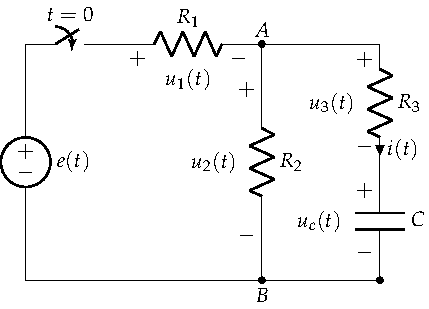
\includegraphics{figs/BT5_CondicionesIniciales_condensador.pdf}}
\end{minipage}
\begin{minipage}{0.5\linewidth}
  Datos:

  $e(t) = 10\unit{\volt}$
  
  $R_1 = R_2 = 2 \unit{\ohm}$

  $R_3= 4 \unit{\ohm}$

  $C = 1 \unit{\farad}$
\end{minipage}

\subsubsection*{Solución}

\begin{enumerate}
\item

  En $t < 0$, dado que el circuito lleva funcionando un tiempo
  indefinido, el condensador se comporta como un circuito
  abierto. Además, el interruptor está abierto y, por tanto, la fuente
  está aislada del circuito. En estas condiciones
  $u_c(0^-) = \qty{0}{\volt}$. Debido a las condiciones de
  continuidad, $u_c(0^+) = u_c(0^-) = \qty{0}{\volt}$.

\begin{minipage}{0.6\linewidth}
  Con este resultado podemos determinar el resto de tensiones del
  circuito en $t = 0^+$, teniendo en cuenta que para $t > 0$ el
  interruptor está cerrado y el condensador es equivalente a un
  cortocircuito ($u_c(0^+) = \qty{0}{\volt}$).
\end{minipage}
\begin{minipage}{0.4\linewidth}
  \center{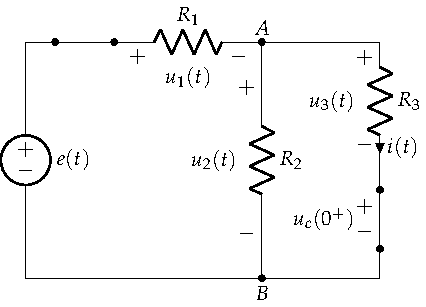
\includegraphics{figs/BT5_CondicionesIniciales_condensador0+.pdf}}
\end{minipage}

En este circuito $R_2$ y $R_3$ están en paralelo entre sí, siendo
$R_{23} = \frac{R_2 \cdot R_3}{R_2 + R_3}$. Esta resistencia paralelo
está en serie con $R_1$, formando un divisor de tensión. Por tanto:

\begin{align*}
  u_2(0^+) = u_3(0^+) &= e(t) \cdot \frac{R_{23}}{R_1 + R_{23}} = \qty{4}{\volt}\\
  u_1(0^+) &= e(t) - u_2(0^+) = \qty{6}{\volt}.
\end{align*}

\item

  Analizamos ahora el circuito para $t > 0$, en el que el interruptor
  está abierto.


  \begin{minipage}{0.6\linewidth}
    La resistencia vista por el condensador es

  \[
    R_{th} = R_3 + \frac{R_1 \cdot R_2}{R_1 + R_2} = \qty{5}{\ohm}
  \]

  Por tanto:
  \begin{equation*}
    \tau = \frac{C}{G_{th}} = \qty{5}{\second}
  \end{equation*}
\end{minipage}
\begin{minipage}{0.4\linewidth}
  \center{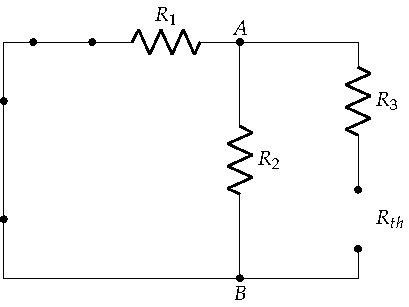
\includegraphics{figs/BT5_CondicionesIniciales_condensador_Rth.pdf}}
\end{minipage}

Obtenemos la respuesta forzada analizando el circuito en régimen
permanente, en el que el condensador se comportará como un circuito
abierto:

\begin{equation*}
  u_{C}(\infty) = e(t) \cdot \frac{R_2}{R_1 + R_2} = \qty{5}{\volt}
\end{equation*}

Obtenemos la respuesta natural apagando la fuente $e(t)$:

\begin{equation*}
  u_{Cn}(t) = A \cdot e^{-0.2t}
\end{equation*}

Para obtener la constante $A$ recurrimos a la condición inicial
$u_C(0^+) = \qty{0}{\volt}$:

\begin{equation*}
  A = u_C(0^+) - u_C(\infty) = \qty{-5}{\volt}
\end{equation*}

Por tanto:

\begin{equation*}
  u_C(t) = 5 - 5 \cdot e^{-0.2t} \unit{\volt}
\end{equation*}

\item Con este resultado podemos obtener la corriente que circula por
  el condensador:

\begin{equation*}
  i_C(t) = C \cdot \diff{u_C}{t} = e^{-0.2t} \unit{\ampere}
\end{equation*}

y las tensiones en las resistencias:

\begin{align*}
  u_{R3}(t) &=  R_3 \cdot i_C(t) = 4 \cdot e^{-0.2t} \unit{\volt}\\
  u_{R2}(t) &=  u_{R3}(t) + u_C(t) = 5 - e^{-0.2t} \unit{\volt}
\end{align*}
  


  
  
\end{enumerate}

\clearpage

\subsection{}

Calcular la corriente $i(t)$ para $t > 0$.

\begin{minipage}{0.5\textwidth}
  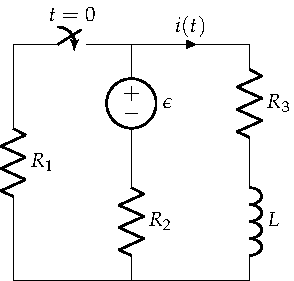
\includegraphics{figs/FM_4_2}
\end{minipage}
\hfill
\begin{minipage}{0.5\textwidth}
  Datos:
  \begin{align*}
    \epsilon &= \SI{24}{\volt}\\
    R_1 &= \SI{8}{\ohm}\\
    R_2 &= \SI{4}{\ohm}\\
    R_3 &= \SI{4}{\ohm}\\
    L &= \SI{15}{\henry}
  \end{align*}
\end{minipage}

\subsubsection*{Solución}

Calculamos las condiciones iniciales ($t = 0^-$)

Dibujamos el circuito para $t < 0$ y obtenemos:

\begin{minipage}{0.3\textwidth}
  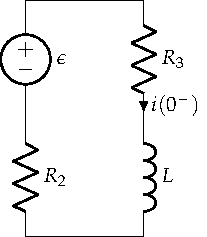
\includegraphics{figs/FM_4_2_t0-}
\end{minipage}
\begin{minipage}{0.7\textwidth}
  \begin{equation*}
    i(t) = \frac{\epsilon}{R_2 + R_3}
  \end{equation*}
\end{minipage}

Por tanto, $i(0^-) = \SI{3}{\ampere}$. Al tratarse de una bobina,
$i(0^+) = i(0^-) = \SI{3}{\ampere}$.

A continuación dibujamos el circuito para $t > 0$ para obtener la
respuesta natural y la respuesta forzada.

Para obtener la respuesta natural apagamos las fuentes. En este
circuito obtenemos:

\begin{minipage}{0.3\textwidth}
  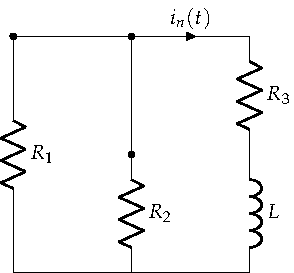
\includegraphics{figs/FM_4_2_natural}
\end{minipage}
\begin{minipage}{0.7\textwidth}
  \begin{align*}
    R_{th} &= R_3 + R_1||R_2 = 20/3\si{\ohm}\\
    \tau &= L/R_{th} = 9/4\si{\second}\\
    i_n(t) &= A \cdot e^{-\frac{t}{\tau}} = A \cdot e^{-4t/9}
  \end{align*}
\end{minipage}
Queda por determinar la constante de integración.

Para obtener la respuesta forzada volvemos a activar las fuentes. En
este circuito obtenemos:

\begin{minipage}{0.3\textwidth}
  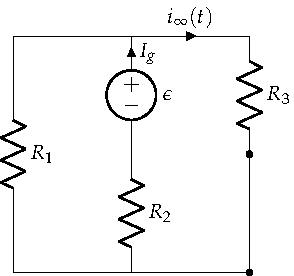
\includegraphics{figs/FM_4_2_forzada}
\end{minipage}
\begin{minipage}{0.7\textwidth}
  \begin{align*}
    I_g &= \frac{\epsilon}{R_2 + R_1||R_3}\\
    i_\infty(t) &= I_g \cdot \frac{G_3}{G_3 + G_1} = \SI{2.4}{\ampere}
  \end{align*}
\end{minipage}

Con estos dos resultados podemos obtener la respuesta completa:

\begin{align*}
  i(t) &= i_n(t) + i_\infty(t)\\
  i(t) &= A \cdot e^{-4t/9} + 2.4
\end{align*}

Para determinar la constante de integración recurrimos a las
condiciones iniciales:

\begin{align*}
  i(0^+) &= A + 2.4\\
  i(0^+) &= 3\\
  A &= 0.6
\end{align*}

Por tanto,

\begin{equation*}
  i(t) = 0.6 \cdot e^{-4t/9} + 2.4
\end{equation*}

\clearpage

\subsection{}

Calcular la tensión en bornes del condensador para $t > 0$.

\begin{minipage}{0.5\textwidth}
  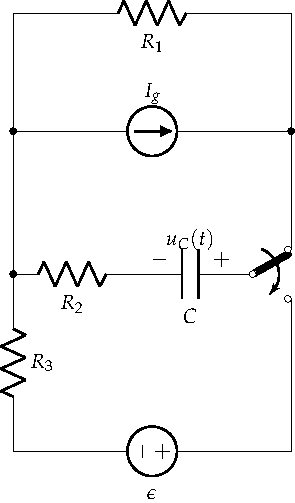
\includegraphics[scale=0.85]{figs/FM_4_3}
\end{minipage}
\hfill
\begin{minipage}{0.5\textwidth}
  Datos:
  \begin{align*}
    \epsilon &= \SI{20}{\volt}\\
    I_g &= \SI{4}{\ampere}\\
    R_1 &= \SI{6}{\ohm}\\
    R_2 &= \SI{4}{\ohm}\\
    R_3 &= \SI{12}{\ohm}\\
    C &= \SI[parse-numbers=false]{1/16}{\farad}      
  \end{align*}

\end{minipage}

\subsubsection*{Solución}

Calculamos las condiciones iniciales ($t = 0^-$)

Dibujamos el circuito para $t < 0$ y obtenemos:

\begin{minipage}{0.3\textwidth}
  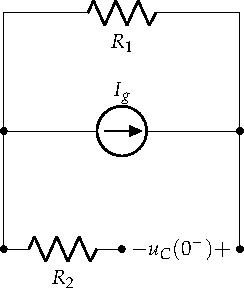
\includegraphics{figs/FM_4_3_t0-}
\end{minipage}
\begin{minipage}{0.7\textwidth}
  \begin{equation*}
    u_C(t) = I_g \cdot R_1 
  \end{equation*}
\end{minipage}

Por tanto, $u_c(0^-) = \SI{24}{\volt}$. Al tratarse de un condensador,
$u_C(0^+) = u_C(0^-) = \SI{24}{\volt}$.

A continuación dibujamos el circuito para $t > 0$ para obtener la
respuesta natural y la respuesta forzada.

Para obtener la respuesta natural apagamos las fuentes. En este
circuito obtenemos:

\begin{minipage}{0.3\textwidth}
  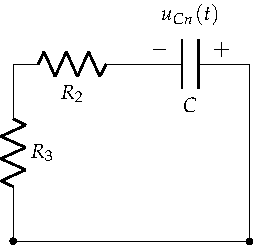
\includegraphics{figs/FM_4_3_natural}
\end{minipage}
\begin{minipage}{0.7\textwidth}
  \begin{align*}
    R_{th} &= R_2 + R_3 = \SI{16}{\ohm}\\
    \tau &= C/G_{th} = \SI{1}{\second}\\
    u_{Cn}(t) &= A \cdot e^{-\frac{t}{\tau}} = A \cdot e^{-t}
  \end{align*}
\end{minipage}
Queda por determinar la constante de integración.

Para obtener la respuesta forzada volvemos a activar las fuentes. En
este circuito obtenemos:

\begin{minipage}{0.3\textwidth}
  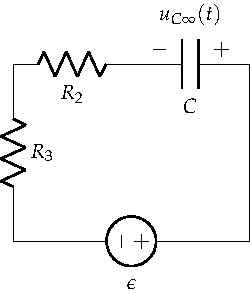
\includegraphics{figs/FM_4_3_forzada}
\end{minipage}
\begin{minipage}{0.7\textwidth}
  \begin{equation*}
    u_{c\infty}(t) = \epsilon = \SI{20}{\volt}
  \end{equation*}
\end{minipage}

Con estos dos resultados podemos obtener la respuesta completa:

\begin{align*}
  u_C(t) &= u_{Cn}(t) + u_{c\infty}(t)\\
  u_C(t) &= A \cdot e^{-t} + 20
\end{align*}

Para determinar la constante de integración recurrimos a las
condiciones iniciales:

\begin{align*}
  u_C(0^+) &= A + 20\\
  u_C(0^+) &= 24\\
  A &= \SI{4}{\volt}
\end{align*}

Por tanto,

\begin{equation*}
  u_C(t) = 4 \cdot e^{-t} + 20
\end{equation*}

\clearpage

\subsection{}

Determina las corrientes $i_L(t)$ e $i_1(t)$ para $t > 0$.

\begin{minipage}{0.7\textwidth}
  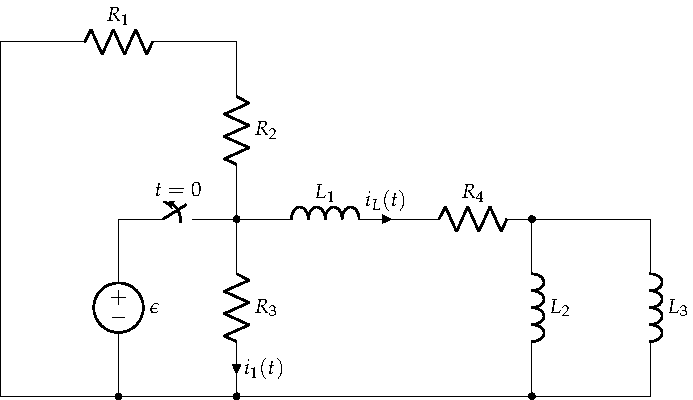
\includegraphics{figs/HKD84}
\end{minipage}
\hfill
\begin{minipage}{0.3\textwidth}
  Datos:
  \begin{align*}
    \epsilon &= \SI{18}{\volt}\\
    R_1 &= \SI{120}{\ohm}\\
    R_2 &= \SI{60}{\ohm}\\
    R_3 &= \SI{90}{\ohm}\\
    R_4 &= \SI{50}{\ohm}\\
    L_1 &= \SI{1}{\milli\henry}\\
    L_2 &= \SI{2}{\milli\henry}\\
    L_3 &= \SI{3}{\milli\henry}
  \end{align*}
\end{minipage}

\subsubsection*{Solución}

Calculamos las condiciones iniciales ($t = 0^-$)

Dibujamos el circuito para $t < 0$:

\begin{center}
  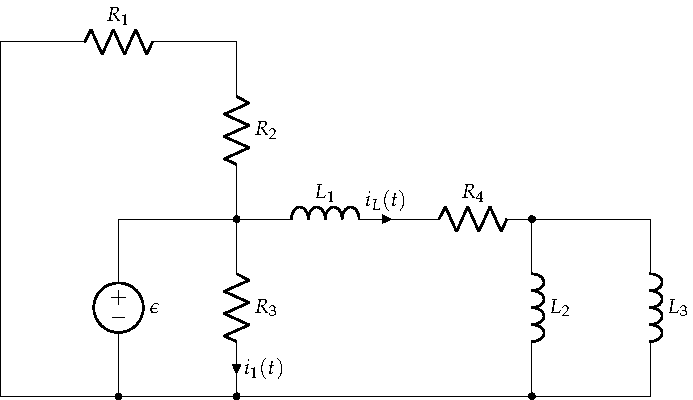
\includegraphics[scale=0.85]{figs/HKD84_t0-}
\end{center}

Obtenemos:
\begin{equation*}
  i_L(t) = \frac{\epsilon}{R_4} = \SI{360}{\milli\ampere}
\end{equation*}

Al tratarse de una bobina,
$i_L(0^+) = i_L(0^-) = \SI{360}{\milli\ampere}$.

En este circuito podemos calcular
$i_1(0^-) = \frac{\epsilon}{R_3} = \SI{200}{\milli\ampere}$. Este
valor nos servirá de referencia cuando calculemos $i_1(t)$.

A continuación dibujamos el circuito para $t > 0$ para obtener la
respuesta natural y la respuesta forzada. En el circuito resultante no
hay fuentes, por lo que únicamente tendremos respuesta natural.

\begin{center}
  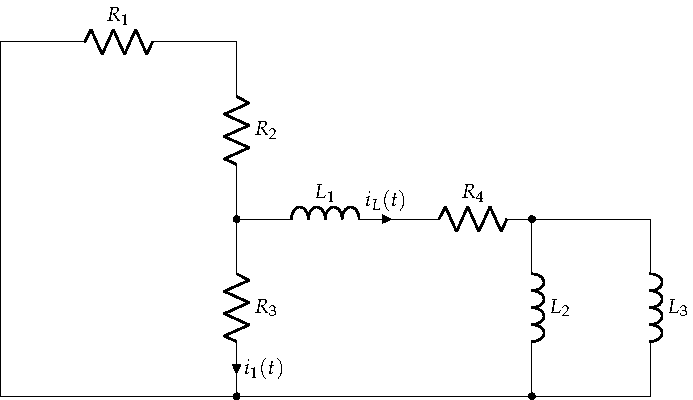
\includegraphics{figs/HKD84_natural}
\end{center}

  \begin{align*}
    L_{eq} &= L_1 + L_2||L_3 = \SI{2.2}{\milli\henry}\\
    R_{th} &= (R_1 + R_2) || R_3 + R_4  = \SI{110}{\ohm}\\
    \tau &= L_{eq}/R_{th} = \SI{20}{\micro\second}\\
    i_{Ln}(t) &= A \cdot e^{-\frac{t}{\tau}} = A \cdot e^{-5 \cdot 10^{-4} \cdot t}
  \end{align*}

  Queda por determinar la constante de integración. Dado que la
  respuesta forzada es 0 podemos calcular directamente esta constante
  con la respuesta natural y las condiciones iniciales:


\begin{align*}
  i_L(t) &= i_{Ln}(t) = A \cdot e^{-5 \cdot 10^{-4} \cdot t}\\
  i_L(0^+) &= A = 0.36
\end{align*}

Por tanto,

\begin{equation*}
  i_L(t) = 0.36 \cdot e^{-5 \cdot 10^{-4} \cdot t}\si{\ampere}
\end{equation*}

Para calcular la corriente $i_1(t)$ usamos un divisor de corriente a
partir de $i_L(t)$:

\begin{equation*}
  i_1(t) = -i_L(t) \cdot \frac{1/R_3}{1/R_3 + 1/(R_1 + R_2)} = -0.24 \cdot e^{-5 \cdot 10^{-4} \cdot t}\si{\ampere}
\end{equation*}

En el primer apartado habíamos obtenido
$i_1(0^-) = \SI{200}{\milli\ampere}$. Con esta ecuación obtenemos
$i_1(0^+) = -\SI{240}{\milli\ampere}$. Los valores no coinciden porque
en una resistencia no hay condición de continuidad.

\clearpage

\section{Transitorio de segundo orden}

\subsection{}

El circuito de la figura ha alcanzado el régimen permanente con el
interruptor cerrado. El interruptor se abre en $t = 0$. Calcula las
expresiones de la tensión en bornes del condensador y de la corriente
por la bobina para $t > 0$.

\vspace*{1cm}

\begin{minipage}{0.7\textwidth}
  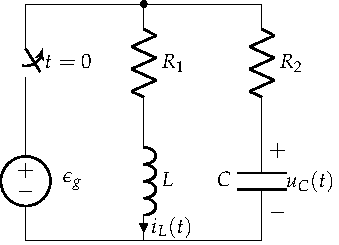
\includegraphics[scale=0.95]{figs/FM_4_8}
\end{minipage}
\hfill
\begin{minipage}{0.3\textwidth}
  Datos:
  \begin{align*}
    \epsilon_g &= \SI{10}{\volt}\\
    R_1 &= \SI{10}{\ohm}\\
    R_2 &= \SI{5}{\ohm}\\
    L &= \SI{2.5}{\henry}\\
    C &= \SI{0.2}{\farad}      
  \end{align*}
\end{minipage}

\subsection*{Solución}

Calculamos las condiciones iniciales ($t = 0^-$)

Dibujamos el circuito para $t < 0$ y obtenemos:

\begin{minipage}{0.3\textwidth}
  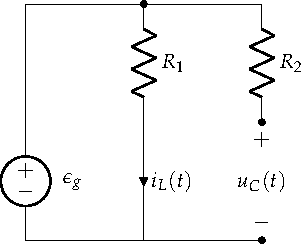
\includegraphics{figs/FM_4_8_t0-}
\end{minipage}
\begin{minipage}{0.7\textwidth}
  \begin{align*}
    u_C(t) &= \SI{10}{\volt}\\
    i_L(t) &= \frac{\epsilon_g}{R_1} = \SI{1}{\ampere}
  \end{align*}
\end{minipage}

\bigskip Por tanto, $u_c(0^+) = u_c(0^-) = \SI{10}{\volt}$ y
$i_L(0^+) = i_L(0^-) = \SI{1}{\ampere}$.

A continuación dibujamos el circuito para $t > 0$ para obtener la
respuesta natural y la respuesta forzada. En el circuito resultante no
hay fuentes, por lo que no habrá respuesta forzada.

\begin{minipage}{0.3\textwidth}
  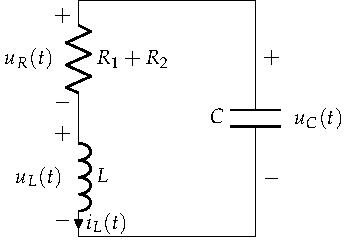
\includegraphics{figs/FM_4_8_natural}
\end{minipage}
\begin{minipage}{0.7\textwidth}
  \begin{align*}
    \alpha &= \frac{R}{2L} = \SI{3}{\per\second}\\
    \omega_0 &= \frac{1}{\sqrt{LC}} = \sqrt{2}\si{\radian\per\second}
  \end{align*}
\end{minipage}

\bigskip

Dado que $\alpha > \omega_0$ se trata de un transitorio
sobreamortiguado:

\begin{align*}
  s_1 &= -\alpha + \sqrt{\alpha^2 - \omega_0^2} = \SI{-0.354}{\per\second}\\
  s_2 &= -\alpha - \sqrt{\alpha^2 - \omega_0^2} = \SI{-5.645}{\per\second}\\
  i_L(t) &= A_1 \cdot e^{-0.354 \cdot t} + A_2 \cdot e^{-5.645 \cdot t}
\end{align*}

Para determinar las constantes de integración recurrimos a las
condiciones iniciales:

\bigskip

\begin{minipage}{0.3\textwidth}
  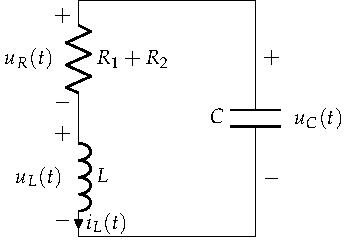
\includegraphics[scale=0.8]{figs/FM_4_8_natural}
\end{minipage}
\begin{minipage}{0.7\textwidth}
  \begin{align*}
    u_R(t) + u_L(t) &= u_C(t)\\
    u_L(0^+) &= u_C(0^+) - u_R(0^+)\\
    u_R(0^+) &= R \cdot i_L(0^+) = \SI{15}{\volt}\\
    u_L(0^+) &= 10 - 15 = \SI{-5}{\volt}
  \end{align*}
\end{minipage}

\bigskip

Por tanto,

\begin{align*}
  i_L(0^+) &= \SI{1}{\ampere}\\
  \diff{i_L(t)}{t}{t = 0^+} &= \frac{1}{L} \cdot u_L(0^+) = \SI{-2}{\ampere\per\second}
\end{align*}

Con estos resultados, particularizamos la ecuación de $i_L(t)$ para
$t = 0$ y así planteamos las ecuaciones para obtener $A_1$ y $A_2$:

\begin{align*}
  i_L(0^+) &= A_1 + A_2 = 1\\
  \diff{i_L(t)}{t}{t = 0^+} &= A_1 \cdot s_1 + A_2 \cdot s_2 = -2
\end{align*}

Por tanto,

\begin{align*}
  A_1 &= 0.689\\
  A_2 &= 0.311
\end{align*}

Finalmente,

\begin{equation*}
  i_L(t) = 0.689 \cdot e^{-0.354 \cdot t} + 0.311 \cdot e^{-5.645 \cdot t}\\
\end{equation*}

Para obtener la tensión en el condensador recurrimos a la LKV:

\begin{align*}
  u_C(t) &= u_R(t) + u_L(t) = \\
         &= R \cdot i_L(t) + L \diff{i_L(t)}{t} = \\
         &= 9.7275 \cdot e^{-0.354 \cdot t} + 0.275 \cdot e^{-5.645 \cdot t}
\end{align*}

\clearpage

\subsection{}

En el circuito de la figura, calcula la tensión $u_c(t)$ para $t > 0$.

\vspace*{1cm}

\begin{minipage}{0.7\textwidth}
  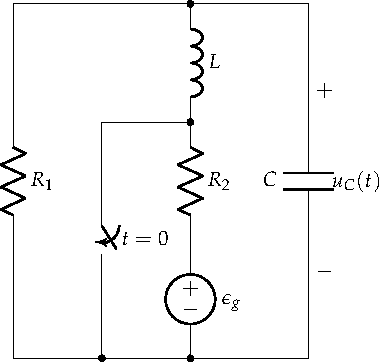
\includegraphics{figs/FM_4_9}
\end{minipage}
\hfill
\begin{minipage}{0.3\textwidth}
  Datos:
  \begin{align*}
    \epsilon_g &= \SI{4}{\volt}\\
    R_1 &= \SI{2}{\ohm}\\
    R_2 &= \SI{2}{\ohm}\\
    L &= \SI{2}{\henry}\\
    C &= \SI{0.25}{\farad}      
  \end{align*}
\end{minipage}

\subsection*{Solución}

Calculamos las condiciones iniciales ($t = 0^-$). Dibujamos el
circuito para $t < 0$ y obtenemos:

\bigskip

\begin{minipage}{0.3\textwidth}
  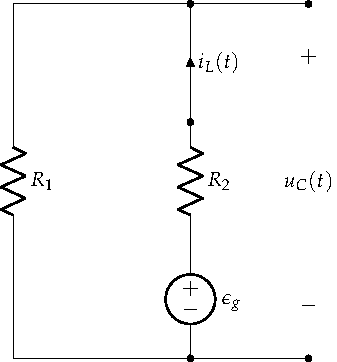
\includegraphics[scale=0.8]{figs/FM_4_9_t0-}
\end{minipage}
\begin{minipage}{0.7\textwidth}
  \begin{align*}
    u_C(t) &= \SI{2}{\volt}\\
    i_L(t) &= \frac{\epsilon_g}{R_1 + R_2} = \SI{1}{\ampere}
  \end{align*}
\end{minipage}

\bigskip Por tanto, $u_c(0^+) = u_c(0^-) = \SI{2}{\volt}$ y
$i_L(0^+) = i_L(0^-) = \SI{1}{\ampere}$.

A continuación dibujamos el circuito para $t > 0$ para obtener la
respuesta natural y la respuesta forzada. En el circuito resultante no
hay fuentes, por lo que no habrá respuesta forzada.

\bigskip

\begin{minipage}{0.3\textwidth}
  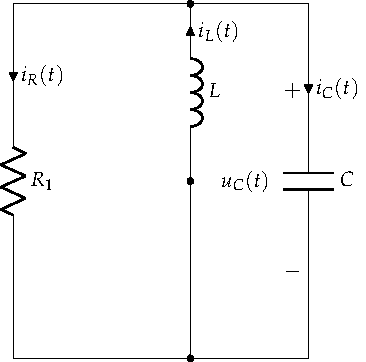
\includegraphics[scale=0.8]{figs/FM_4_9_natural}
\end{minipage}
\begin{minipage}{0.7\textwidth}
  \begin{align*}
    \alpha &= \frac{G}{2C} = \SI{1}{\per\second}\\
    \omega_0 &= \frac{1}{\sqrt{LC}} = 2\si{\radian\per\second}
  \end{align*}
\end{minipage}

\bigskip

Dado que $\alpha < \omega_0$, se trata de un transitorio
subamortiguado:

\begin{align*}
  \omega_d &= \sqrt{\omega_0^2 - \alpha^2} = \sqrt{3}\si{\radian\per\second}\\
  u_C(t) &= (B_1 \cdot \cos(\sqrt{3} \cdot t) + B_2 \cdot \sin(\sqrt{3} \cdot t)) \cdot e^{-t}
\end{align*}

Para determinar las constantes de integración recurrimos a las
condiciones iniciales:

\bigskip

\begin{minipage}{0.3\textwidth}
  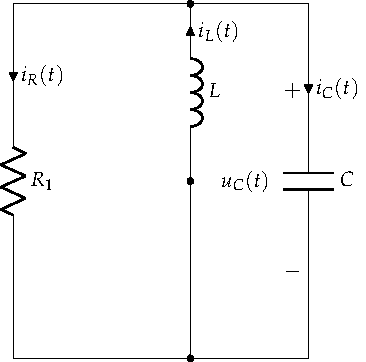
\includegraphics[scale=0.8]{figs/FM_4_9_natural}
\end{minipage}
\begin{minipage}{0.7\textwidth}
  \begin{align*}
    i_C(0^+) &= i_L(0^+) - i_R(0^+)\\
    i_R(0^+) &= G_1 \cdot u_C(0^+) = \SI{1}{\ampere}\\
    i_C(0^+) &= 1 - 1 = \SI{0}{\ampere}
  \end{align*}
\end{minipage}

\bigskip

Por tanto,

\begin{align*}
  u_C(0^+) &= \SI{2}{\volt}\\
  \diff{u_C(t)}{t}{t = 0^+} &= \frac{1}{C} \cdot i_C(0^+) = \SI{0}{\volt\per\second}
\end{align*}

Con estos resultados, particularizamos la ecuación de $u_C(t)$ para
$t = 0$ y así planteamos las ecuaciones para obtener $B_1$ y $B_2$:

\begin{align*}
  u_C(0^+) &= B_1 = 2\\
  \diff{u_C(t)}{t}{t = 0^+} &= -e^{-t} \cdot (2\cos(\sqrt{3}t) + B_2\sin(\sqrt{3}t)) +\\
           &+ e^{-t} \cdot (-2\sqrt{3}\sin(\sqrt{3}t) + \sqrt{3} B_2\cos(\sqrt{3}t)) =\\
           &= 0
\end{align*}

Por tanto,

\begin{align*}
  B_1 &= 2\\
  B_2 &= \frac{2\sqrt{3}}{3}
\end{align*}

Finalmente,

\begin{equation*}
  u_C(t) = (2 \cdot \cos(\sqrt{3} \cdot t) + \frac{2\sqrt{3}}{3} \cdot \sin(\sqrt{3} \cdot t)) \cdot e^{-t}
\end{equation*}


\clearpage

\end{document}
